% VLDB template version of 2020-03-05 enhances the ACM template, version 1.7.0:
% https://www.acm.org/publications/proceedings-template
% The ACM Latex guide provides further information about the ACM template

\documentclass{article}
\usepackage{listings}
\usepackage[margin=20mm]{geometry}
\usepackage{graphicx}
\usepackage{amsfonts}
\usepackage{amsmath}
\usepackage{physics}
\usepackage{parskip}
\usepackage{enumitem}
\usepackage{cancel}

%% The following content must be adapted for the final version
% paper-specific
\newcommand\vldbdoi{XX.XX/XXX.XX}
\newcommand\vldbpages{XXX-XXX}
% issue-specific
\newcommand\vldbvolume{14}
\newcommand\vldbissue{1}
\newcommand\vldbyear{2020}
% should be fine as it is
\newcommand\vldbauthors{\authors}
\newcommand\vldbtitle{\shorttitle} 
% leave empty if no availability url should be set
\newcommand\vldbavailabilityurl{http://vldb.org/pvldb/format_vol14.html}
\newcommand\oname{\operatorname}

\newtheorem{theorem}{Teor.}
\newtheorem{definition}{Def.}
\newtheorem{example}{Ej.}
\newtheorem{excercise}{Ejer.}

\begin{document}

\textbf{Ex. 5.1: }

Ommited so far. Involves assigning numerical degrees of belief in diverse affirmations. Will re-visit though.

\textbf{Ex. 5.2: }From these equations, find the exact conditions on $(x,\,y,\,a,\,b)$ for divergence on the probability scale; that is,
\begin{align*}
	\abs{P(S|DI_X)-P(S|DI_Y)}>\abs{P(S|I_X)-P(S|I_Y)}.
\end{align*}

\textbf{Answer:}

The equations Edwin is refering to concern the proposition $S$ that a certain drug is safe, with data $D$ that a certain Mr. N claimed in T.V. that the drug is unsafe. Then, Mr. X and Mr. Y both have the same degree of trust in Mr. N:
\begin{align*}
	P(D|SI_X)&=P(D|SI_Y)=a,\\
	P(D|\overline{S}I_X)&=P(D|\overline{S}I_Y)=b.
\end{align*}

Here $a<b$ makes Mr. N more likely to be telling the truth. They however differ on their initial degree of trust in the drug's safety:
\begin{align*}
	P(S|I_X)&=x,\\
	P(S|I_Y)&=y,
\end{align*}
which finaly leads to
\begin{align*}
	P(S|DI_X)&=\frac{ax}{ax+b(1-x)},\\
	P(S|DI_Y)&=\frac{ay}{ay+b(1-y)}.
\end{align*}

The condition for divergence is thus, in these terms:
\begin{align*}
	\abs{\frac{ax}{ax+b(1-x)}-\frac{ay}{ay+b(1-y)}}&>\abs{x-y}.
\end{align*}

The special case $a=b$, where Mr. N is completely untrustworthy and conveys no information on his data, we get (as seen in the book), that the data changes nothing on Mr. X and Mr. Y's opinion. This equation reflects this by having no solution: rather than converging or diverging, they remain unchanged.

In the other cases, some mathsages lead to the expresion
\begin{align*}
	ab&>\abs{(ax+b(1-x))(ay+b(1-y))}.
\end{align*}

The value inside the absolute value is quadratic on $x$ and $y$, and symmetric. We're thus dealing with a conic section symmetric about axes rotated $45°$ w.r.t. the original pair of cartesian axes. This can be resolved analitically, but I'm not sure there's much purpose. Turns out to be four hyperbolas, with foci in $(0, 0)$ and another point along the $\oname{span}(1, 1)$ axis which depends on $a$ and $b$.

Figure \ref{fig:5.2} shows the convergence and divergence regions for $a<b$ (Mr. N being kinda trustworthy) and $a>b$, the ratio $a/b$ controling the exentricity.

\begin{figure}[h]
	\center
	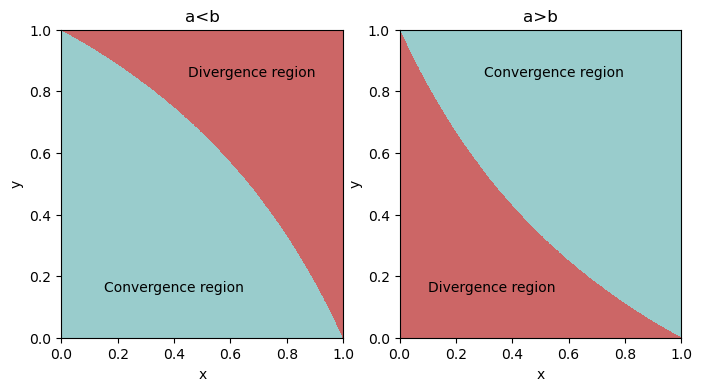
\includegraphics[width=0.6\textwidth]{Numerical/5.2.png}
	\caption{Regions of convergence and divergence for a liar Mr. N (left) and a not so liar Mr. N (right).}
	\label{fig:5.2}
\end{figure}

In the case where Mr. N is seen as trustworthy, they region of convergence is that of general agreement in that the drug is unsafe, their opinions diverging if they both believe the drug to be safe. The opposite happens whenever Mr. N is seen as a liar in general. They converge if they already kinda agreed that the pill was safe. I expected the divergence region to measure lack of agreement...

\textbf{Ex. 5.3: }It is evident from ($5.31$) that Mr. X and Mr. Y can never experience a reversal of viewpoint; that is, if initially Mr. X believes more strongly than Mr. Y in the safety of the drug, this will remain true whatever the values of $a$, $b$. Therefore, a necessary condition for reversal must be that they have different conditions about Mr. N; $a_x\neq a_y$ and/or $b_x\neq b_y$. But this does not prove that reversal is actually possible, so more analysis is needed. If reversal is possible, find a sufficient condition on $(x,\,y,\,a_x,\,a_y,\,b_x,\,b_y)$ for this to take place, and illustrate it by a verbal scenario like the above. If it is not possible, prove this and explain the intuitive reason why reversal cannot happen.

\textbf{Answer:}

The equations for the log posterior for the drug being safe now take the form
\begin{align*}
	\log\left[\frac{P(S|DI_X)}{P(\overline{S}|DI_X)}\right]&=\log\left[\frac{x}{1-x}\right]+\log\left[\frac{a_X}{b_X}\right],\\
	\log\left[\frac{P(S|DI_Y)}{P(\overline{S}|DI_Y)}\right]&=\log\left[\frac{y}{1-y}\right]+\log\left[\frac{a_Y}{b_Y}\right],
\end{align*}
so that their difference is
\begin{align*}
	\log\left[\frac{x}{1-x}\right]-\log\left[\frac{y}{1-y}\right]+\log\left[\frac{a_X}{b_X}\right]-\log\left[\frac{a_Y}{b_Y}\right].
\end{align*}

So, inversion of beliefs is acchieved by requiring that the difference of log likelihoods be greater in magnitude than the difference of original beliefs, with opposite sign. For the sake of concreteness, if $x=0.6$ and $y=0.4$, it suffices to take $a_Y/b_Y>0.6$ and $a_X/b_X<0.4$. Say, $a_Y=b_X=0.8$, $b_Y=a_X=0.2$; this takes an original degree of belief from (log prior) $0.81$ to $-1.96$.

In this example, Mr. X's belief is that the drug is most probably safe, and Mr. Y's is the opposite. But Mr. X is so convinced that Mr. N wouldn't lie, and Mr. Y is so convinced of the contrary, that their stances after this encounter become reversed. Cool.

\textbf{Ex. 5.4: }Our story has a curious sequel. In turn, it was noticed that Neptune was not following exactly its proper course, and so one naturally assumed that there is still another planet causing this. Percivall Lowel, by a similar calculation, predicted its orbit, and Clyde Tombaugh proceeded to find the new planet (Pluto), although not so close to the predicted position. But now the story changes: modern data on the motion of Pluto's moon indicated that the mass of Pluto is too small to have caused the perturbation of Neptune which motivated Lowell's calculation. Thus, the discrepancies in the motions of Neptune and Pluto were unaccounted for (We are indebted to Dr. Brad Schaeter for this information). Try to extend our probability analysis to take this new circumstance into account; at this point, where did Newton's theory stand? For more background information, see Hoyt (1980) or Whyte (1980). More recently, it appears that the mass of Pluto had been estimated wrongly and the discrepancies were after all not reall; then it seems that the status of Newton's theory should revert to its former one. Discuss this sequence of pieces of information in terms of probability theory. Do we update by Bayes' theorem as each new fact comes in? Or do we just return to the beginning when we learn that a previous datum was false?

\end{document}
\endinput
